\subsection{Módulo genérico de las barreras ferroviarias}
	\label{sec:ACG_lc}
	
	El módulo \textit{LevelCrossing} (ver Figura \ref{fig:GeneralSystem}) es el encargado de implementar el funcionamiento de las barreras ferroviarias en los pasos a nivel. El ACG utiliza la información otorgada por el RNA para determinar cuál es el \textit{netElement} donde se sitúa el paso a nivel y cuales son los \textit{netElements} mas próximos, para que puedan reportar su estado al módulo \textit{LevelCrossing}. Además, el ACG implementa todas las conexiones para cada una de las rutas en las cuales el paso a nivel sea condición necesaria para su habilitación. El diagrama de bloques de la máquina de estados finitos con camino de datos diseñado para lograr este objetivo se muestra en la Figura \ref{fig:LCB_module}.
	
	\begin{figure}[H]
		\centering
		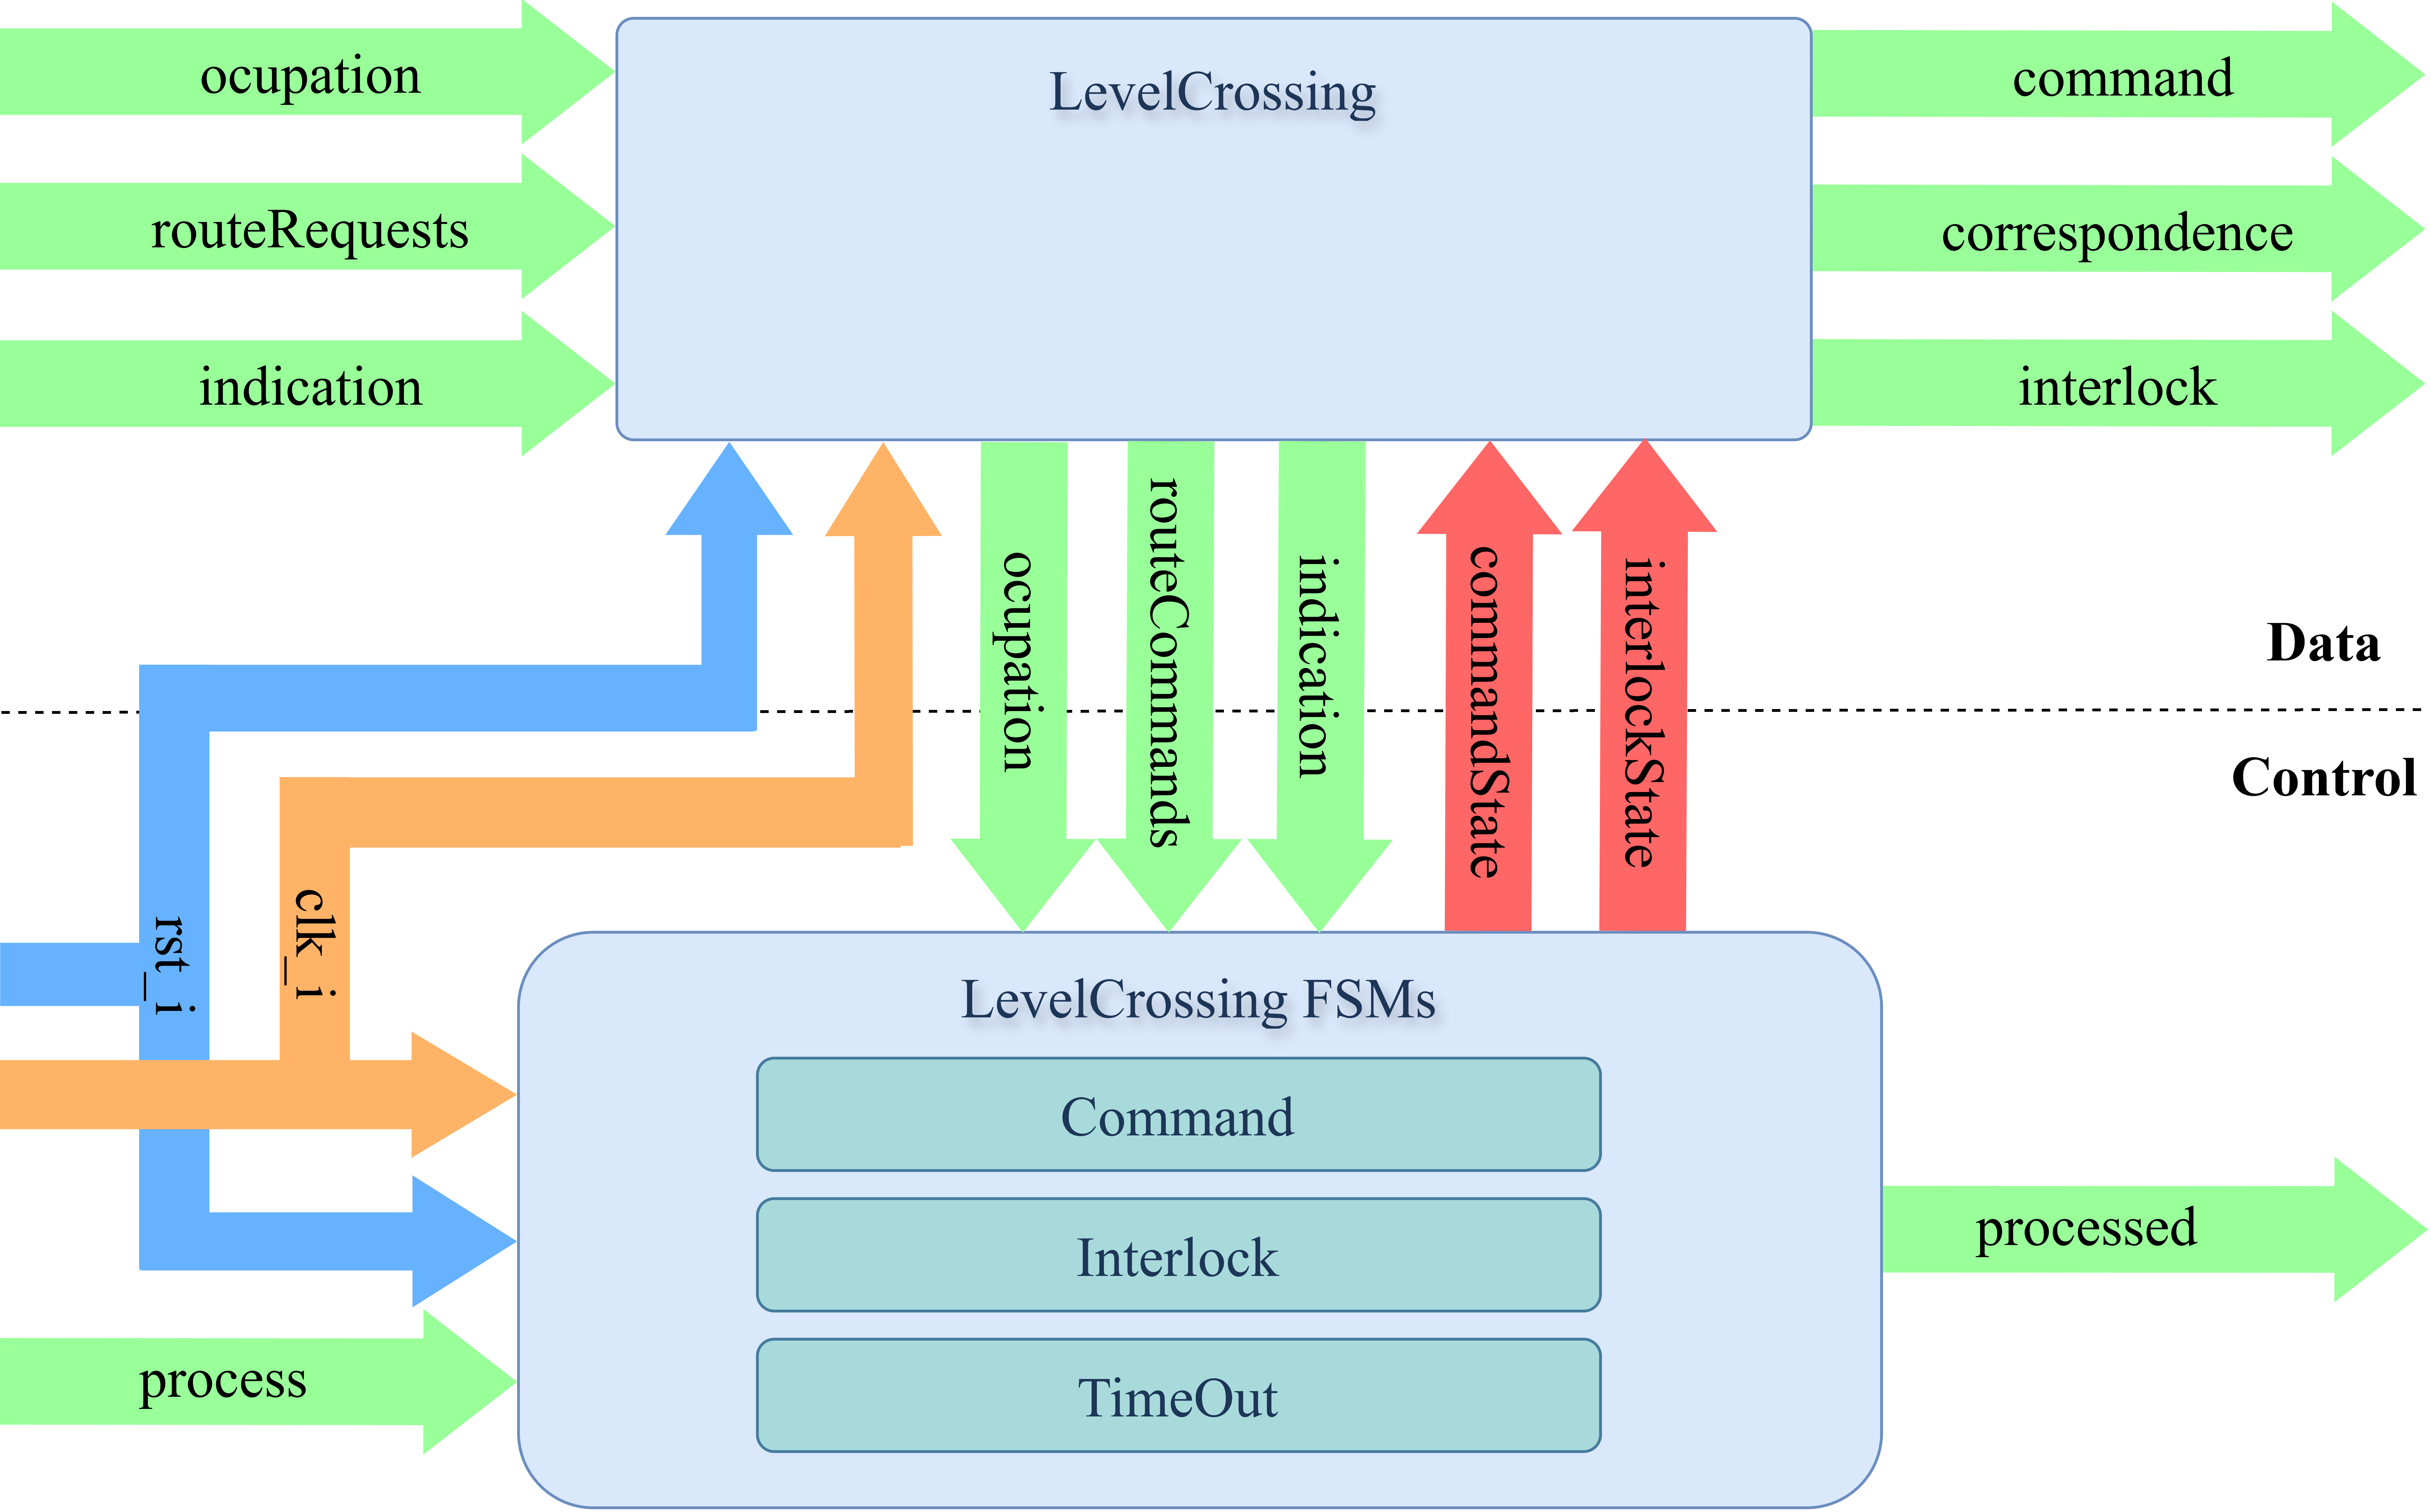
\includegraphics[width=1\textwidth]{Figuras/LCB_module}
		\centering\caption{FSMD del módulo genérico de \textit{LevelCrossing}.}
		\label{fig:LCB_module}
	\end{figure}
	
	Tal como se explicó en la Sección \ref{sec:switches}, las barreras ferroviarias también poseen comando, indicación y correspondencia: comando para controlar la barrera, indicación para reportar su estado actual al módulo \textit{LevelCrossing} y correspondencia para declarar su estado final a la ruta que lo solicite. Además, el ACG implementa todas las conexiones necesarias a todas las rutas que tengan a la barrera en cuestión como condición necesaria de habilitación. Finalmente, el módulo \textit{LevelCrossing} tiene una salida que define su estado de enclavamiento frente a otras rutas que lo requieran.
	
	El comportamiento de una barrera de paso a nivel genérico se define en la red de Petri de la Figura \ref{fig:LCB_Petri}. Una barrera se mantendrá en estado alto a menos que una ruta solicite que el brazo de barrera descienda o si los \textit{netElements} cercanos se encuentran ocupados. Durante la transición se espera la confirmación de que la barrera ha descendido mientras se mantiene la ocupación para terminar el movimiento en el estado bajo, estado en el cual solo podrá salir si la ocupación termina y ninguna ruta solicita que la barrera se mantenga baja.
	
	\begin{figure}[H]
		\centering
		\includegraphics[width=1\textwidth]{Figuras/LCB_petri}
		\centering\caption{Red de Petri del modelo dinámico de \textit{LevelCrossing}.}
		\label{fig:LCB_Petri}
	\end{figure}
	
	Durante el estado de transición la barrera tendrá 7 segundos para llegar al estado bajo. Al cumplirse este tiempo, si la indicación y el comando no coinciden y los \textit{netElements} cercanos se encuentran libres, la barrera volverá al estado alto. Esto impide que el sistema habilite rutas cuando los actuadores de algún elemento se atascan o su indicación es diferente al comando que se ha enviado. La confirmación de la indicación otorga un grado de seguridad mayor al no asumir que un comando enviado implica automáticamente que al actuador se le impone dicho estado.